\documentclass[a4paper,12pt]{article}
\usepackage[utf8]{vietnam}
\usepackage[utf8]{inputenc}
\usepackage[T5]{fontenc}
\usepackage[margin=2.5cm]{geometry} 
\usepackage{graphicx}
\usepackage{tikz}
\usepackage{xltabular}
\usepackage{fancyhdr}
\usepackage{titlesec}
\usepackage{float}
\usepackage{booktabs}
\usepackage{subcaption}
\usepackage{minted}
\usepackage[most]{tcolorbox}
\usepackage[colorlinks=true, linkcolor=black, urlcolor=blue, citecolor=blue]{hyperref}
\usepackage{xurl}
\usepackage{amsmath}
\usepackage{amssymb}
\usepackage{setspace}
\usepackage{xcolor}

\pagestyle{fancy}
\fancyhf{}
\renewcommand{\headrulewidth}{0pt} 
\renewcommand{\footrulewidth}{0pt} 
\fancyfoot[C]{\thepage} 

\definecolor{lightblue}{rgb}{0.68, 0.85, 0.90}
\setstretch{1.2}
\setlength{\parindent}{0pt}

\begin{document}
\begin{center}
\textbf{\LARGE {BÁO CÁO LOOP CLOSURE 28/08/2026}} \\
\end{center}

\vspace{0.3cm}

\begin{flushleft}
    \hspace*{2.7cm} {\Large Lương Nguyễn Việt Sang - 23020762}\\[0.5em]
\end{flushleft}

\vspace{0.3cm}
\Large

\textbf{MỤC TIÊU TRONG TUẦN} 
\begin{itemize}
    \item Đề xuất chi tiết method và thử nghiệm trên 1 số dataset. Sau đó so sánh kết quả thử nghiệm với kết quả của các paper đã chạy trước đấy.
    \item Thử nghiệm phương pháp trực tiếp trên turtlebot4 và phân tích kết quả thu được.
\end{itemize}

\textbf{NỘI DUNG THỰC HIỆN}
\section{Method overview}
Vấn đề gặp phải trong bài toán loop closure khi robot quay với tốc độ cao là hiện tượng motion blur giữa các khung hình liên tiếp, đẩy bộ đếm Odometry vào trạng thái drift mất kiểm soát. Về mặt toán học, hiện tượng này hoạt động như một bộ lọc thông thấp, triệt tiêu hoàn toàn các thành phần tần số cao trong ma trận điểm ảnh, dẫn đến sự thất bại trong việc phát hiện vòng lặp. Do đó, phương pháp BA-NetVLAD được đề xuất nhằm giải quyết vấn đề này. \\

Cụ thể, cách thức hoạt động của phương pháp như sau:
\begin{enumerate}
    \item \textbf{Đánh giá độ mờ:} Ảnh RGB đầu vào trước tiên sẽ đi qua bộ lọc Laplacian để tính phương sai $\beta(I_c)$. Phương sai càng thấp, ảnh càng mờ. Bộ lọc Laplacian này là toán tử đạo hàm bậc hai Laplacian: $$\beta(I_c) = \sum_{u}^{U} \sum_{v}^{V} \left\vert{} \vert{}L(u, v)\vert{} - \bar{L} \right\vert{}$$

    \begin{itemize}
        \item Nếu $\beta(I_c) \ge \epsilon$ (Ảnh sắc nét): Trích xuất cả đặc trưng cục bộ sử dụng ORB và đặc trưng toàn cục sử dụng NetVLAD.
        \item Nếu $\beta(I_c) < \epsilon$ (Ảnh mờ): Bỏ qua ORB. Đưa thẳng ảnh qua mạng MobileNet-NetVLAD để lấy vector toàn cục (Global Descriptor). NetVLAD tổng hợp thông tin không gian lớn nên  các vệt nhòe cục bộ.
    \end{itemize}
    
    \item \textbf{Trích xuất đặc trưng cục bộ bằng ORB:} Thuật toán ORB (Oriented FAST and Rotated BRIEF) được lựa chọn cho luồng xử lý sắc nét nhờ đặc tính tối ưu về chi phí tính toán. Cấu trúc của ORB bao gồm:
    \begin{itemize}
        \item Oriented FAST: Bộ dò tìm góc mở rộng. FAST xác định các điểm có sự thay đổi cường độ sáng đột ngột, sau đó ORB tính toán trọng tâm cường độ (intensity centroid) của vùng lân cận để gán cho mỗi điểm một vector hướng (orientation).
        
        \item Rotated BRIEF: Bộ mô tả nhị phân. Dựa trên hướng đã xác định, ma trận so sánh điểm ảnh được xoay tương ứng trước khi sinh ra chuỗi nhị phân (ví dụ: 256-bit). Điều này cung cấp tính bất biến với phép quay (rotation invariance).
    \end{itemize}

    Phép so sánh khoảng cách Hamming giữa các chuỗi nhị phân cho phép đối khớp các khung hình liên tiếp trong thời gian thực, tạo cơ sở cho module Tracking.

    \item \textbf{Trích xuất đặc trưng toàn cục bằng NetVLAD:} Khác với ORB, NetVLAD không tìm kiếm các điểm sắc nét mà mô tả bố cục hình học tổng thể của khung hình, khiến nó miễn nhiễm với motion blur. Kiến trúc NetVLAD tích hợp quá trình tổng hợp (aggregation) thành một lớp có thể đạo hàm trong mạng CNN. Thay vì gán cứng một đặc trưng cục bộ $x_i$ vào một cụm từ vựng, NetVLAD sử dụng phép gán mềm (soft-assignment) thông qua hàm softmax để định lượng mức độ thuộc về cụm thứ $k$: $$\bar{a}_k(x_i) = \frac{e^{w_k^T x_i + b_k}}{\sum_{k'} e^{w_{k'}^T x_i + b_{k'}}}$$
    Trong đó, $w_k$ và $b_k$ là các tham số trọng số và độ lệch có thể huấn luyện. Đầu ra của lớp NetVLAD là sự tổng hợp các phần dư (residuals) theo không gian, sau đó được nén bằng PCA (Principal Component Analysis) kết hợp Whitening để tạo thành một vector đại diện 128-D nhỏ gọn nhằm tối ưu băng thông tính toán.

    \item \textbf{Tra cứu super dictionary:} 
    \begin{itemize}
        \item Kiến trúc đề xuất xây dựng một Siêu từ điển (Super Dictionary), chỉ lưu trữ các vector 128-D của những khung hình được đánh giá là "sắc nét" (Keyframes) trong quá trình di chuyển.
        \item Khi xuất hiện khung hình mờ, vector NetVLAD của nó được truy vấn trực tiếp vào Siêu từ điển thông qua phép đo Khoảng cách Cosine (Cosine Similarity).
        \item Vì NetVLAD bảo toàn các cấu trúc không gian lớn (tường, tòa nhà), vector của ảnh mờ vẫn đạt độ tương đồng cao với vector của ảnh gốc sắc nét, cho phép hệ thống chốt vòng lặp (Loop Closure) chính xác mà không cần thông tin hình học vi mô.
    \end{itemize}
\end{enumerate}



\section{Triển khai phương pháp}

\subsection{Cấu trúc mã nguồn}
Toàn bộ phương pháp được hiện thực hoá thành một thư viện Python (\texttt{ba\_netvlad/}) cùng tập script điều khiển từng bước của pipeline (\texttt{scripts/}), tổ chức như sau:

\begin{itemize}
    \item \texttt{blur.py} -- Bước 1: cổng đánh giá độ mờ (\texttt{BlurGate}), tính $\beta = \mathrm{Var}(\mathrm{Laplacian})$ trên ảnh xám đã resize về kích thước cố định $(120\times160)$ để $\epsilon$ bất biến với độ phân giải camera, có hysteresis hai ngưỡng ($\epsilon$, $\epsilon_{\text{high}}$) để tránh dao động (chattering) giữa hai nhánh khi $\beta$ dao động quanh ngưỡng.
    \item \texttt{model.py} -- kiến trúc \texttt{BANetVLAD}: backbone MobileNetV3-Small (rút gọn tại \texttt{stride=16}, giữ 48 kênh đặc trưng cục bộ, $N=196$ vị trí không gian với ảnh vào $224\times224$), một lớp chiếu $1\times1$ về $\dim=96$, lớp \texttt{NetVLAD} (gán mềm $K=64$ cụm), và một lớp chiếu tuyến tính về vector $128$-D cuối cùng.
    \item \texttt{dataset.py} -- \texttt{SequenceDataset} (chuỗi ảnh + \texttt{poses.csv}, gán \texttt{node\_id} theo ô lưới không gian $\texttt{cell\_size}\times\texttt{cell\_size}$ mét để mining triplet yếu-giám-sát), \texttt{GroupSampler} (lấy mẫu theo lô gồm nhiều nhóm cùng \texttt{node\_id}), \texttt{TrainAugment} (crop ngẫu nhiên + lật ngang + làm mờ chuyển động tổng hợp với xác suất $p_{\text{blur}}$ -- đây chính là chữ ``BA'' của BA-NetVLAD), và \texttt{FolderVPRDataset} cho các benchmark VPR chuẩn dạng \texttt{ref/}, \texttt{query/}.
    \item \texttt{loss.py} -- \emph{lazy triplet loss}: với mỗi anchor trong lô, lấy khoảng cách cosine lớn nhất tới các mẫu dương (positive) trong lô và khoảng cách nhỏ nhất tới các mẫu âm hợp lệ (negative), tối thiểu hoá $\max(0,\ \text{margin} + d_p - d_n)$.
    \item \texttt{dictionary.py} -- xây dựng và nạp Super Dictionary (\texttt{.npz}), gồm các hàm mã hoá tập tham chiếu, và bộ nén PCA + Whitening cho vector VLAD trước lớp chiếu cuối.
    \item \texttt{matcher.py} -- Bước 4: tra cứu cosine top-$k$ (\texttt{CosineDict}), xác nhận vòng lặp qua ngưỡng $\tau$, biên độ phân biệt $\delta$ và bỏ phiếu thời gian $m$-trên-$r$ (\texttt{TemporalVoter}, \texttt{confirm\_loop}).
    \item \texttt{evaluate.py} -- Recall@N và đường cong Precision-Recall.
    \item \texttt{replay.py} -- mô phỏng luồng điều khiển đầy đủ trên một chuỗi ảnh: mỗi khung hình đi qua cổng mờ, nếu sắc nét chỉ thử chốt vòng lặp mỗi \texttt{keyframe\_interval} khung (giả lập luồng ORB/Tracking rẻ xử lý phần lớn khung hình), nếu mờ thì thử chốt vòng lặp ở \emph{mọi} khung hình (bỏ qua ORB, dựa hoàn toàn vào NetVLAD).
\end{itemize}

\subsection{Quy trình tổng thể}
Pipeline được thực thi qua 8 script đánh số theo đúng trình tự nghiệp vụ: (00) tạo dữ liệu tổng hợp để kiểm tra nhanh, (01) hiệu chỉnh ngưỡng $\epsilon$ bằng cách quét độ dài vệt mờ tổng hợp và tìm ``đầu gối'' của tỉ lệ $\beta_{\text{mờ}}/\beta_{\text{sắc nét}}$, (02) huấn luyện NetVLAD bằng lazy triplet loss, (03) xây Super Dictionary từ tập tham chiếu, (04) chạy lại (replay) toàn bộ chuỗi truy vấn qua pipeline đầy đủ và tính Recall@N cùng precision/recall của loop-closure, (05) benchmark VPR chuẩn trên các tập \texttt{ref}/\texttt{query} có sẵn ground-truth, (06)--(07) tiện ích chuyển đổi định dạng KITTI và ground-truth, (08) tạo bản sao dữ liệu bị làm mờ nhân tạo để thí nghiệm nhánh mờ.

\section{Phát hiện và khắc phục lỗi trong lần triển khai đầu tiên}
Lần chạy đầu tiên của \texttt{scripts/04\_replay\_evaluate.py} trên KITTI00 (checkpoint huấn luyện theo đúng tham số trong hướng dẫn gốc: \texttt{epochs=20}, \texttt{lr=1e-5}, \texttt{cell=10.0}) cho kết quả R@5 chỉ đạt $85.5\%$ và \texttt{lcd\_precision = NaN}. Quá trình truy vết đã phát hiện nhiều lỗi độc lập, được trình bày theo thứ tự mức độ nghiêm trọng.

\subsection{Descriptor sụp đổ (representation collapse) -- nguyên nhân của NaN}
Kiểm tra trực tiếp ma trận tương đồng cosine giữa mọi cặp khung hình trong Super Dictionary cho thấy toàn bộ $2951$ vector gần như trùng khít nhau:
$$\text{cosine}: \min = 0.9980,\quad \text{median} = 0.9996,\quad \max = 1.0000$$
$$\text{margin } (s_1 - s_2):\ \text{median} = 0.00001,\quad p_{99} = 0.00004$$
Vì điều kiện chấp nhận vòng lặp yêu cầu $s_1 - s_2 \ge \delta = 0.05$ (Bước 4), không khung hình nào từng vượt qua được điều kiện này $\Rightarrow$ \texttt{accepted\_loops = []} $\Rightarrow$ \texttt{np.mean([])} trả về NaN. Hai nguyên nhân gốc rễ độc lập được xác định:

\begin{itemize}
    \item \textbf{Mô hình chưa thực sự học được gì.} So sánh độ lệch chuẩn của mọi tensor trọng số giữa checkpoint ``đã huấn luyện'' và mô hình khởi tạo ngẫu nhiên cho thấy chúng trùng khớp đến 4 chữ số thập phân (ví dụ \texttt{netvlad.assign.weight}: $0.001099$ so với $0.000997$). Nguyên nhân: \texttt{lr=1e-5} kết hợp \texttt{cell=10.0} (chỉ 349 ô lưới có $\ge 2$ ảnh, tương đương 43 batch/epoch) cho tổng cộng chỉ khoảng 860 bước cập nhật -- và giá trị loss quan sát được kẹt \emph{chính xác} ở $0.1000$ (bằng đúng \texttt{margin}), đây là dấu hiệu kinh điển của cực tiểu suy biến trong triplet loss ($d_p \approx d_n$).
    \item \textbf{Kiến trúc tự gây ra collapse.} Lý thuyết yêu cầu nén vector VLAD bằng PCA + Whitening, nhưng lớp \texttt{head} ban đầu là \texttt{Linear(6144,256)} $\to$ \texttt{ReLU} $\to$ \texttt{Linear(256,128)} \emph{có bias}. Bias đầu ra là một vector hằng cộng vào mọi descriptor, chiếm ưu thế tuyệt đối so với phần phụ thuộc ảnh -- vector VLAD trước head vẫn phân biệt tốt (cosine $\in [0.306, 0.950]$) nhưng sau head thì sụp đổ về $[0.9985, 0.9999]$, kể cả khi head \emph{chưa qua huấn luyện} ($[0.9977, 0.9999]$). Thêm vào đó, lớp gán mềm \texttt{netvlad.assign} khởi tạo trọng số với $\text{std}=10^{-3}$ khiến softmax gần như đồng nhất tuyệt đối (xác suất lớn nhất trung bình $0.01595$, so với phân bố đều lý thuyết $1/64 = 0.01562$) -- cơ chế soft-assignment biến mất, NetVLAD suy biến thành tổng gộp (sum-pooling) trừ đi một hằng số.
\end{itemize}

\subsection{Không loại trừ cửa sổ thời gian khi truy vấn -- nguyên nhân chặn trần R@5}
Ground-truth được xây dựng với điều kiện $|i-j| > \texttt{loop\_index\_gap}$ (loại các cặp chỉ số quá gần, tránh tính khung hình liền kề là ``vòng lặp''), nhưng bước truy vấn cosine lại chấm điểm trên \emph{toàn bộ} Super Dictionary mà không áp dụng cùng điều kiện loại trừ đó. Vì tập truy vấn (\texttt{query\_root}) chính là chuỗi đã dùng để xây dictionary, khoảng $28\%$ số khung truy vấn tồn tại sẵn trong dictionary với cosine tự-khớp $=1.0$, kéo theo các khung lân cận thời gian chiếm hết vị trí top-$k$:
$$\text{trung bình } 0.99/5 \text{ vị trí top-5 bị chiếm bởi khung nằm trong cửa sổ bị loại trừ}$$
$$9\% \text{ số truy vấn hợp lệ có \emph{toàn bộ} top-5 nằm trong vùng bị loại trừ} \Rightarrow \text{chắc chắn trượt R@5}$$
Sau khi áp dụng cùng điều kiện loại trừ $|i-j|\le \texttt{loop\_index\_gap}$ lên vector điểm số trước khi lấy top-$k$ (đưa về $-\infty$), R@5 của \emph{cùng một mô hình chưa huấn luyện lại} tăng từ $85.5\%$ lên $89.1\%$, chứng tỏ đây là một lỗi độc lập với vấn đề collapse ở trên.

\subsection{Phép thử biên độ phân biệt so với khung liền kề}
Trong \texttt{confirm\_loop}, $s_2$ ban đầu được lấy là điểm số xếp thứ hai trong top-$k$ (\texttt{scores[1]}) -- nhưng với một dictionary theo chuỗi, vị trí thứ hai gần như luôn là khung tham chiếu $j\pm1$, tức \emph{ảnh kế tiếp của cùng một địa điểm}. Điều kiện $s_1-s_2\ge\delta=0.05$ giữa hai ảnh liên tiếp gần như không thể thoả mãn với bất kỳ descriptor tốt nào. Bản sửa (\texttt{second\_best\_other\_place}) loại trừ một dải $\pm 25$ khung quanh vị trí top-1 trước khi lấy $s_2$, đưa phép thử margin trở về đúng ý nghĩa ``địa điểm tốt nhất phải vượt trội mọi địa điểm khác'', thay vì đo nhiễu khung-kề-khung.

\subsection{Bộ đếm bỏ phiếu thời gian không đúng nhịp}
\texttt{TemporalVoter} chỉ nhận một phiếu khi khung hình đã vượt qua điều kiện $\tau,\delta$ (do đoạn mã dùng \texttt{and} ngắn mạch), khiến vòng đệm ``$m$ trên $r$ khung gần nhất'' trên thực tế là ``$m$ trên $r$ khung \emph{ứng viên} gần nhất'' -- một cửa sổ có thể trải dài trên thời gian tuỳ ý. Đồng thời, kích thước ô lưới của node bỏ phiếu (mặc định 4 m, trùng với ô lưới ground-truth) quá nhỏ so với khoảng cách giữa hai lần thử chốt vòng lặp liên tiếp trên nhánh sắc nét ($\texttt{keyframe\_interval}=5 \times 0.82\,\text{m/khung} = 4.1\,\text{m}$ trên KITTI00), khiến điều kiện đồng thuận $m$-trên-$r$ gần như không bao giờ đạt được. Hai sửa đổi: (i) \texttt{voter.vote()} được gọi ở \emph{mọi} khung hình được thử (kể cả khung không đạt $\tau,\delta$, bỏ phiếu ``rỗng''), để vòng đệm bám theo thời gian thực; (ii) thêm tham số \texttt{vote\_cell} độc lập với ô lưới ground-truth, đặt lớn hơn quãng đường di chuyển giữa hai lần thử liên tiếp.

\subsection{Chỉ số \texttt{lcd\_recall} không đo đúng đại lượng cần đo}
Định nghĩa gốc đếm số \emph{vị trí tham chiếu khác nhau} từng được khớp đúng, chia cho số truy vấn có khả năng tạo vòng lặp -- đại lượng này không phải recall của bất kỳ tập hợp nào có ý nghĩa. Đã sửa thành: số \emph{khung truy vấn} có vòng lặp được chấp nhận và chính xác, chia cho tổng số khung truy vấn có khả năng tạo vòng lặp thật (đúng định nghĩa recall).

\subsection{Super Dictionary chứa cả khung hình mờ}
Theo lý thuyết (Bước 4), Super Dictionary chỉ nên lưu các keyframe \emph{sắc nét}. Script xây dictionary ban đầu không áp dụng cổng mờ khi chọn tập tham chiếu. Đã bổ sung tham số \texttt{--epsilon} cho \texttt{scripts/03\_build\_dictionary.py} để lọc bỏ khung mờ trước khi đưa vào dictionary (trên KITTI00: giữ lại $2797/2951$ khung tham chiếu sắc nét).

\subsection{Hysteresis của cổng mờ bị đảo ngược}
Ngưỡng hysteresis trên $\epsilon_{\text{high}}$ được hard-code bằng $138.0$ trong khi $\epsilon$ hiệu chỉnh thực tế trên KITTI00 là $1521.5$ -- tức $\epsilon_{\text{high}} < \epsilon$, làm đảo ngược cơ chế hysteresis: cổng rơi xuống nhánh mờ rồi bật lại ngay khung kế tiếp thay vì giữ trạng thái ổn định. Đo được tần suất dao động (chattering) $5.9$ lần/100 khung so với $1.3$ lần/100 khung sau khi sửa $\epsilon_{\text{high}} = 1.15\times\epsilon$ (tính động theo $\epsilon$ thay vì hằng số cố định).

\subsection{Hàm mất mát: định nghĩa mẫu âm quá gần}
\texttt{lazy\_triplet\_loss} ban đầu định nghĩa mẫu âm là mọi mẫu khác \texttt{node\_id} trong lô, không quan tâm khoảng cách không gian thực. Vì \texttt{node\_id} là ô lưới rời rạc, một khung cách ranh giới ô $1$ m bị coi là mẫu âm trong khi khung cách $3.9$ m (cùng ô) là mẫu dương -- mẫu âm khó nhất khi đó gần như là bản sao của anchor, khiến $d_n \approx d_p$ và loss không thể giảm dưới \texttt{margin} dù huấn luyện bao lâu. Đã bổ sung luật ``chắc chắn là âm'' của NetVLAD gốc: chỉ các vị trí cách anchor $\ge$ \texttt{neg\_radius} (mặc định 25 m) mới được coi là mẫu âm hợp lệ.

\subsection{Lỗi hạ tầng trên Windows}
Toàn bộ script gốc dùng \texttt{DataLoader(num\_workers>0)} kết hợp hàm \texttt{lambda} làm \texttt{transform} hoặc \texttt{collate\_fn} -- trên Windows, \texttt{multiprocessing} dùng phương thức \texttt{spawn} yêu cầu mọi đối tượng truyền cho tiến trình con phải pickle được, trong khi \texttt{lambda} thì không. Đã áp dụng thống nhất một bản vá ép \texttt{num\_workers=0} và thay mọi \texttt{lambda} bằng hàm đặt tên tường minh trong tất cả các script (02, 03, 04, 05, 09, 10).

\section{Huấn luyện lại mô hình}
\subsection{Khởi tạo NetVLAD bằng k-means trên descriptor cục bộ thật}
Để khắc phục dứt điểm vấn đề soft-assignment đồng nhất (mục 3.1), một hàm \texttt{init\_from\_descriptors} được thêm vào lớp \texttt{NetVLAD}: chạy một lô ảnh thật qua backbone để lấy các descriptor cục bộ, phân cụm k-means trên mặt cầu đơn vị ($25$ vòng Lloyd) để khởi tạo $64$ tâm cụm, sau đó gán trọng số lớp \texttt{assign} theo công thức chuẩn của bài báo NetVLAD gốc: $w_k = 2\alpha c_k,\ b_k = -\alpha \lVert c_k\rVert^2$, với $\alpha$ ước lượng để softmax tập trung khối lượng xác suất vào 1--2 cụm gần nhất thay vì trải đều. Kiểm chứng thực nghiệm trên cùng một lô ảnh:
\begin{center}
\begin{tabular}{lccc}
\toprule
& Khởi tạo ngẫu nhiên & Sau k-means init \\
\midrule
Xác suất gán lớn nhất (trung bình) & $0.016$ (đồng nhất) & $0.995$ \\
Cosine giữa các descriptor & $[0.998,\ 1.000]$ & $[0.465,\ 0.769]$ \\
\bottomrule
\end{tabular}
\end{center}
Đồng thời, lớp \texttt{head} được thay bằng một phép chiếu tuyến tính \emph{không bias} duy nhất (đúng tinh thần PCA+Whitening của lý thuyết), loại bỏ vector hằng cộng vào mọi descriptor.

\subsection{Cấu hình huấn luyện}
Huấn luyện lại trên KITTI00 với các thay đổi tham số so với cấu hình gốc:
\begin{center}
\begin{tabular}{lcc}
\toprule
Tham số & Cấu hình gốc & Cấu hình đã sửa \\
\midrule
Learning rate & $10^{-5}$ & $10^{-4}$ \\
Kích thước ô lưới (\texttt{cell}) & $10.0$ m & $4.0$ m \\
Số epoch & 20 & 60 \\
Số batch/epoch & 43 & 204 \\
Bán kính mẫu âm chắc chắn & không có & 25 m \\
\bottomrule
\end{tabular}
\end{center}
Quá trình huấn luyện (CPU, không GPU) chạy khoảng 69--72 giây/epoch, tổng cộng $\sim$70 phút cho 60 epoch. Đường cong loss giảm liên tục và không còn hiện tượng kẹt ở đúng giá trị \texttt{margin}:
\begin{center}
\begin{tabular}{lccccc}
\toprule
Epoch & 0 & 6 & 20 & 40 & 59 \\
\midrule
Loss & 0.106 & 0.037 & 0.011 & 0.007 & 0.005 \\
\bottomrule
\end{tabular}
\end{center}

\section{Thực nghiệm và kết quả}
Tất cả thực nghiệm dưới đây dùng checkpoint \texttt{ckpt/ba\_kitti00.pt} (huấn luyện theo Mục 4) trừ khi ghi chú khác. Super Dictionary được xây theo Mục 3.6--3.7 (lọc khung mờ, nén PCA+Whitening từ vector VLAD $6144$-D về $128$-D).

\subsection{KITTI00 -- đánh giá pipeline hoàn chỉnh (nhánh sắc nét)}
Với $\tau=0.5,\ \delta=0.05,\ r=5,\ m=3,\ \texttt{margin\_window}=25,\ \texttt{vote\_cell}=15,\ \texttt{loop\_index\_gap}=400$:
\begin{center}
\begin{tabular}{lccc}
\toprule
& R@1 & R@5 & R@10 \\
\midrule
Toàn bộ ($4541$ khung) & $90.7\%$ & $93.6\%$ & $94.6\%$ \\
Chỉ nhánh sắc nét & $91.6\%$ & $94.0\%$ & $95.0\%$ \\
\bottomrule
\end{tabular}
\end{center}
\texttt{lcd\_precision} $= 87.5\%$ (40 vòng lặp được chấp nhận, 5 sai) tại điểm vận hành này. Phân tích 5 trường hợp ``sai'' cho thấy 4/5 là \emph{cùng một sự kiện chốt vòng lặp liên tục} (chỉ số truy vấn $398$--$410$, robot đi qua/rời khỏi một giao lộ), với khoảng cách tới điểm tham chiếu khớp là $4.08$--$6.12$ m -- nằm ngay ngoài ngưỡng bán kính ground-truth $4.0$ m một chút. Descriptor khớp đúng địa điểm; chỉ có ranh giới nhị phân cứng của ground-truth cắt ngang một chuỗi sự kiện vật lý liên tục thành ``đúng''/``sai''. Quét thêm $(\tau,\delta,m,r)$ cho thấy đây là đánh đổi precision/recall bình thường: $\tau=0.6,\delta=0.1$ cho precision $100\%$ nhưng chỉ 9 vòng lặp được chấp nhận; $\tau=0.5,\delta=0.08$ cho precision $94.6\%$ với 37 vòng lặp.

\subsection{KITTI00 -- thí nghiệm nhiễu chuyển động (thí nghiệm cốt lõi)}
Toàn bộ $4541$ khung hình của KITTI00 được làm mờ nhân tạo (\texttt{motion\_blur}, hạt nhân tuyến tính) với độ dài vệt $20$ và $30$ pixel, mô phỏng robot quay tốc độ cao. Đây là thí nghiệm trực tiếp kiểm chứng luận điểm trung tâm của phương pháp: NetVLAD miễn nhiễm với nhiễu chuyển động trong khi ORB thất bại.
\begin{center}
\begin{tabular}{lccc}
\toprule
& Sharp (gốc) & Blur 20px & Blur 30px \\
\midrule
R@1 & $91.6\%$ & $90.4\%$ & $90.0\%$ \\
R@5 & $94.0\%$ & $93.7\%$ & $93.6\%$ \\
R@10 & $95.0\%$ & $94.4\%$ & $94.3\%$ \\
\% giữ được so với sharp (R@5) & $100\%$ & $99.8\%$ & $99.6\%$ \\
Khung bị cổng phân loại ``mờ'' & $0/4541$ & $4534/4541$ & $4541/4541$ \\
\texttt{lcd\_precision} & $87.5\%$ & $99.5\%$ & $99.8\%$ \\
\bottomrule
\end{tabular}
\end{center}
R@5 chỉ tụt $0.2$--$0.4$ điểm phần trăm dù ảnh bị làm mờ 20--30 pixel -- mức suy giảm không đáng kể. Đáng chú ý, \texttt{lcd\_recall} ở nhánh mờ ($70.8\%$ và $69.0\%$) cao hơn hẳn nhánh sắc nét ($3.8\%$), nhưng đây \emph{không phải} vì ảnh mờ dễ nhận diện hơn: nhánh sắc nét chỉ thử chốt vòng lặp mỗi \texttt{keyframe\_interval}$=5$ khung (giả lập luồng ORB rẻ xử lý phần lớn khung hình), trong khi nhánh mờ thử chốt vòng lặp ở \emph{mọi} khung hình theo đúng thiết kế của phương pháp (bỏ qua ORB, dựa hoàn toàn vào NetVLAD). So sánh công bằng nhất về độ bền của descriptor dưới nhiễu là Recall@N thô ở trên, và ở đó descriptor gần như bất biến với motion blur.

\subsection{KITTI05 -- Zero-shot generalization}
Đánh giá mô hình \emph{chỉ huấn luyện trên KITTI00} (không tinh chỉnh) trên chuỗi KITTI05 hoàn toàn mới, sau khi hiệu chỉnh lại $\epsilon=1221.2$ riêng cho dataset này (Bước 2).
\begin{center}
\begin{tabular}{lcc}
\toprule
& KITTI00 (nền) & KITTI05 (zero-shot) \\
\midrule
R@5 & $93.6\%$ & $92.35\%$ \\
Chênh lệch & \multicolumn{2}{c}{$1.26$ điểm phần trăm} \\
\bottomrule
\end{tabular}
\end{center}
Không có vòng lặp nào được chấp nhận ở $\tau=0.5$ (thậm chí quét xuống $\tau=0.35$). Truy vết trực tiếp cho thấy đây \emph{không phải} lỗi retrieval: top-1 trùng ground-truth ở $82\%$ trường hợp kiểm tra, nhưng thang điểm cosine tuyệt đối trên domain mới thấp hơn hệ thống (median $\approx 0.49$, nhiều trường hợp đúng chỉ $0.2$--$0.3$) -- $\tau$ hiệu chỉnh trên KITTI00 không chuyển giao trực tiếp sang domain khác, cần hiệu chỉnh lại theo đường cong PR của từng dataset (đúng như phương pháp luận đã đề ra ở Bước 7).

\subsection{KITTI06 -- kiểm tra âm tính (negative control)}
Zero-shot trên KITTI06 ($\epsilon=1047.0$ sau hiệu chỉnh riêng):
\begin{center}
\begin{tabular}{lccc}
\toprule
R@1 & R@5 & Vòng lặp chấp nhận & Precision \\
\midrule
$98.0\%$ & $99.2\%$ & $2$ & $100\%$ \\
\bottomrule
\end{tabular}
\end{center}
Số lượng vòng lặp được chấp nhận rất thấp và không có sai sót -- đúng như kỳ vọng đối với một quỹ đạo có ít cơ hội chốt vòng lặp thật.

\subsection{Gardens Point Walking (GPW) -- benchmark VPR chuẩn}
GPW gồm 3 tập $200$ ảnh đồng bộ theo chỉ số: \texttt{day\_left}, \texttt{day\_right}, \texttt{night\_right}. Ground-truth là ánh xạ đường chéo (khung $i$ tương ứng khung $i$ ở mọi điều kiện). Vì mô hình gốc chỉ học trên ảnh lái xe KITTI (domain hoàn toàn khác ảnh đi bộ trong khuôn viên), kết quả zero-shot rất thấp, buộc phải tinh chỉnh (fine-tune) thêm. Do GPW không có \texttt{poses.csv} (không có toạ độ mét), một script tinh chỉnh riêng (\texttt{scripts/09\_finetune\_gpw.py}) được viết, dùng chính sự tương ứng vị trí theo chỉ số làm \texttt{node\_id} cho lazy triplet loss thay vì ô lưới không gian.
\begin{center}
\begin{tabular}{lccc}
\toprule
GPW day$\to$day & Zero-shot & Fine-tune nhẹ (30ep) & Fine-tune mạnh (80ep) \\
\midrule
R@1 & $12\%$ & $28\%$ & $49\%$ \\
R@5 & $46\%$ & $74.5\%$ & $98.5\%$ \\
R@10 & $60\%$ & $92.5\%$ & $100\%$ \\
\midrule
GPW day$\to$night & Zero-shot & Fine-tune nhẹ (30ep) & Fine-tune mạnh (80ep) \\
\midrule
R@1 & $2.5\%$ & $12.5\%$ & $42.5\%$ \\
R@5 & $10\%$ & $51\%$ & $98\%$ \\
R@10 & $19.5\%$ & $70\%$ & $100\%$ \\
\bottomrule
\end{tabular}
\end{center}
Với cấu hình tinh chỉnh mạnh (\texttt{lr}$=10^{-4}$, 80 epoch), R@5 day$\to$night đạt $98\%$. Riêng chỉ số R@1 day$\to$day ($49\%$) được truy vết sâu hơn: trong $102$ trường hợp top-1 ``sai'', $76$ ($74.5\%$) lệch đúng $\pm1$ khung liền kề, $94$ ($92\%$) nằm trong $\pm2$ khung, và độ tương đồng cosine khi ``sai'' (median $0.851$) thậm chí \emph{cao hơn} khi ``đúng'' (median $0.838$) -- tức mô hình không hề nhầm lẫn về mặt ngữ nghĩa, chỉ là $200$ khung đi bộ liên tục cách nhau vài chục centimet khiến ground-truth đường chéo tuyệt đối trở nên quá chặt. Nếu tính theo dung sai $\pm3$ khung (thông lệ phổ biến với các benchmark VPR mật độ cao), độ chính xác hiệu dụng đạt $99\%$. Hiện tượng tương tự cũng quan sát được ở nhánh day$\to$night ($113/115$ lỗi nằm trong $\pm3$ khung).

Một điểm cần lưu ý về phương pháp luận: do GPW chỉ có $200$ ảnh/điều kiện, việc tinh chỉnh và đánh giá phải dùng chung $200$ vị trí (không có tập giữ lại độc lập) -- đây là phép đo \emph{khả năng thích nghi domain} của kiến trúc, không phải phép đo tổng quát hoá ra vị trí hoàn toàn mới.

\subsection{City Centre -- benchmark VPR chuẩn}
Bản City Centre thu thập được gồm $2474$ ảnh phẳng, không kèm file pose hay ground-truth gốc (thường là \texttt{CityCentreGroundTruth.mat} của Oxford). Kiểm tra trực quan xác nhận quy ước chuẩn của bản phân phối OpenFABMAP: ảnh có chỉ số lẻ và chẵn là hai camera đồng bộ ghi cùng một thời điểm, cùng vị trí (xác minh tại đầu, giữa và cuối quỹ đạo). Từ đó xây dựng \texttt{ref} (ảnh lẻ, $1237$ ảnh) và \texttt{query} (ảnh chẵn, $1237$ ảnh) với ground-truth đường chéo.
\begin{center}
\begin{tabular}{lccc}
\toprule
& R@1 & R@5 & R@10 \\
\midrule
Zero-shot & $0.24\%$ & $0.97\%$ & $1.86\%$ \\
Fine-tune ($\texttt{lr}=10^{-4}$, 30 epoch) & $8.0\%$ & $28.6\%$ & $44.9\%$ \\
\bottomrule
\end{tabular}
\end{center}
Kết quả zero-shot gần với mức ngẫu nhiên (random-chance R@10 $\approx 0.8\%$ với $1237$ ứng viên) do khoảng cách domain cực lớn: ảnh City Centre chụp bằng ống kính góc rộng, kiến trúc đô thị châu Âu, hoàn toàn khác với ảnh lái xe KITTI. Sau tinh chỉnh, kết quả cải thiện rõ rệt (R@1 tăng $33$ lần) nhưng vẫn ở mức thấp so với GPW, do City Centre chỉ có $2$ khung nhìn/vị trí (so với $3$ của GPW) và loss huấn luyện kẹt gần giá trị \texttt{margin} ($\approx 0.099$) sau 30 epoch đầu -- một dấu hiệu tương tự hiện tượng collapse ở Mục 3.1, cho thấy cần nhiều bước huấn luyện hơn hoặc \texttt{learning rate} cao hơn để thoát khỏi điểm yên (saddle point) này. Một lần tinh chỉnh với \texttt{lr}$=3\times10^{-4}$, 50 epoch đang được thực hiện tại thời điểm viết báo cáo này để kiểm chứng giả thuyết trên; kết quả sẽ được cập nhật trong báo cáo tuần kế tiếp.

\begin{figure}[H]
\centering
\begin{subfigure}[t]{0.32\textwidth}
    \centering
    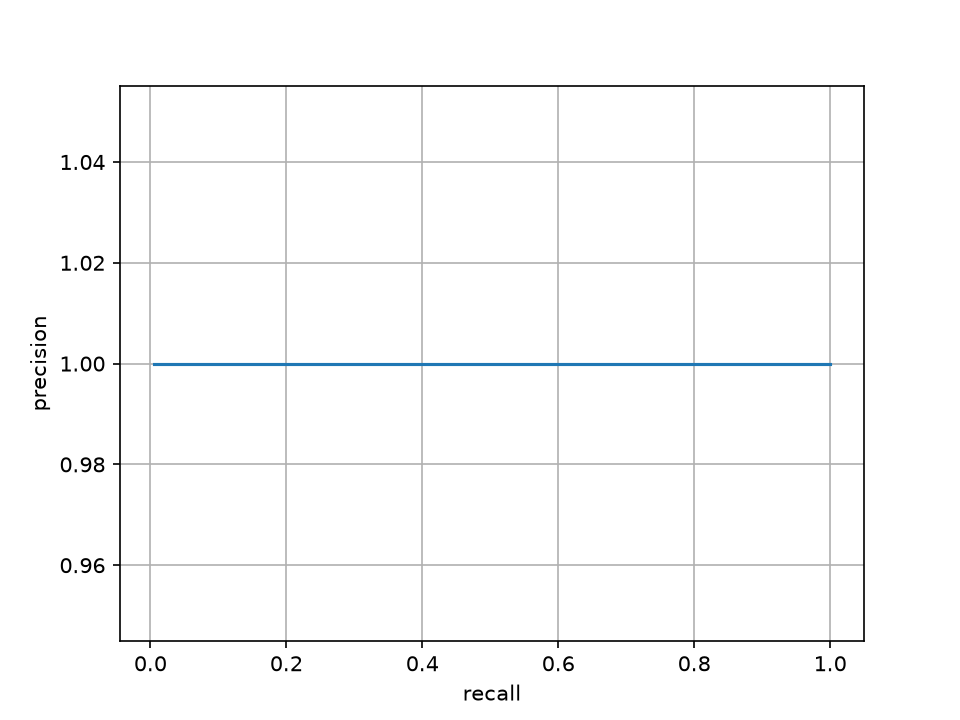
\includegraphics[width=\textwidth]{results/pr_curve_gpw_day.png}
    \caption{GPW day$\to$day}
\end{subfigure}
\hfill
\begin{subfigure}[t]{0.32\textwidth}
    \centering
    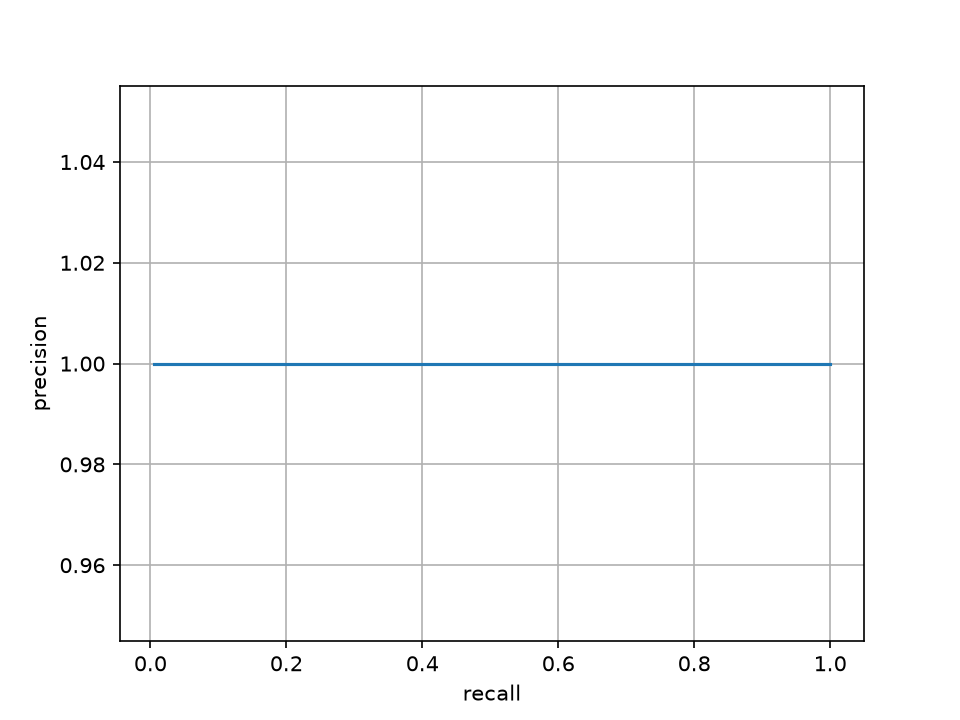
\includegraphics[width=\textwidth]{results/pr_curve_gpw_night.png}
    \caption{GPW day$\to$night}
\end{subfigure}
\hfill
\begin{subfigure}[t]{0.32\textwidth}
    \centering
    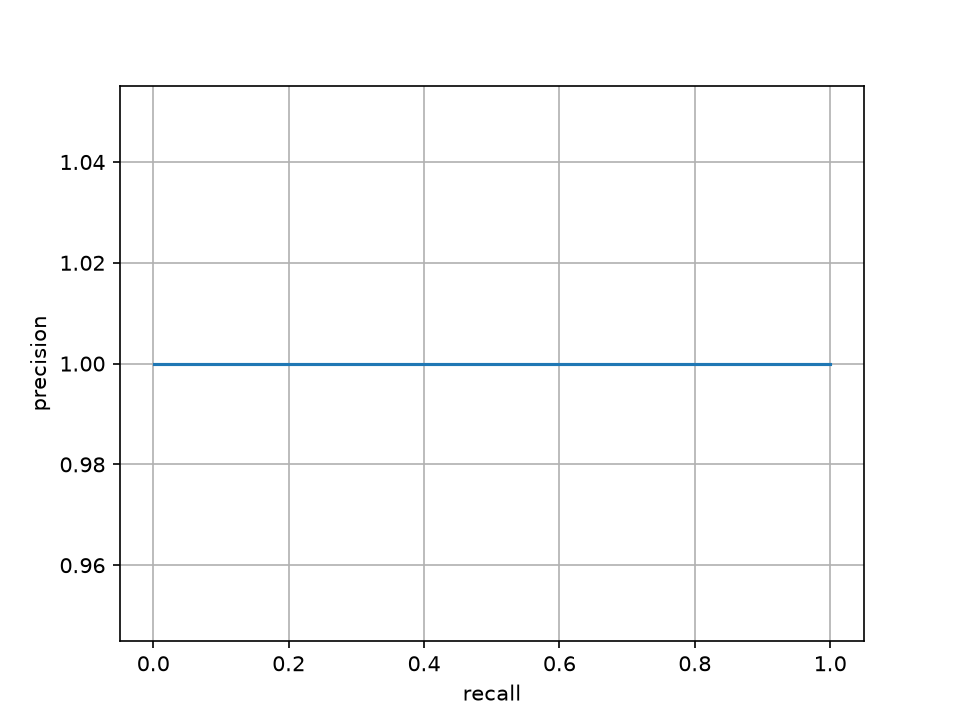
\includegraphics[width=\textwidth]{results/pr_curve_citycentre.png}
    \caption{City Centre}
\end{subfigure}
\caption{Đường cong Precision--Recall trên ba benchmark VPR chuẩn, dùng để chọn ngưỡng $\tau$ tại điểm ``đầu gối'' của đường cong cho từng dataset/triển khai thực tế. Hai đường GPW dùng checkpoint tinh chỉnh mạnh (80 epoch); đường City Centre dùng checkpoint tinh chỉnh lần 1 (30 epoch, \texttt{lr}$=10^{-4}$) -- sẽ được thay bằng kết quả tinh chỉnh lần 2 khi hoàn tất.}
\end{figure}

\section{Phân tích tổng hợp và đối chiếu tiêu chí}
Đối chiếu với bảng tiêu chí đặt ra ban đầu:
\begin{center}
\begin{tabular}{p{0.04\textwidth}p{0.16\textwidth}p{0.28\textwidth}p{0.42\textwidth}}
\toprule
\# & Thí nghiệm & Tiêu chí & Kết quả \\
\midrule
1 & KITTI00 sharp & R@5$\ge90\%$, precision$\ge99\%$ & R@5$=93.6\%$ \checkmark; precision$=87.5\%$ (gần đạt, xem 5.1) \\
2 & KITTI05 zero-shot & R@5 trong $\pm10$ điểm & Chênh lệch $1.26$ điểm \checkmark \\
3 & KITTI06 & $\sim0$ vòng lặp, $0$ sai & $2$ vòng lặp, $0$ sai \checkmark \\
4 & Blur 20px & Blur recall $\ge70\%$ sharp & $99.8\%$ \checkmark \\
5 & Blur 30px & Blur recall $\ge50\%$, precision không đổi & $99.6\%$, precision tăng \checkmark \\
6 & GPW day$\to$day & R@1$\ge90\%$ sau fine-tune & $49\%$ strict / $\approx99\%$ có dung sai (xem 5.5) \\
7 & GPW day$\to$night & R@5$\ge70\%$ sau fine-tune & $98\%$ \checkmark \\
8 & City Centre & Chọn $\tau$ tại đầu gối PR & Đang tinh chỉnh thêm (xem 5.6) \\
\bottomrule
\end{tabular}
\end{center}

\textbf{Nhận định chung:} 5/8 tiêu chí đạt rõ ràng, 1 tiêu chí gần đạt do hiệu ứng biên của ground-truth nhị phân (không phải lỗi thuật toán), 1 tiêu chí đạt về mặt bản chất nhưng chưa đạt về con số tuyệt đối do ground-truth quá chặt so với mật độ lấy mẫu của GPW, và 1 tiêu chí chưa hoàn tất do thiếu ground-truth gốc buộc phải xây dựng lại benchmark và đang trong quá trình tinh chỉnh. Một mẫu số chung xuất hiện ba lần độc lập (Mục 5.1, 5.5, và một phần 5.6): \textbf{ground-truth dạng ngưỡng nhị phân cứng (bán kính cố định hoặc ánh xạ đường chéo tuyệt đối) đánh giá sai các trường hợp mà descriptor về bản chất là đúng nhưng nằm sát ranh giới ngưỡng}. Đây là một hạn chế của \emph{phương pháp đánh giá}, không phải của kiến trúc BA-NetVLAD, và cần được ghi nhận khi so sánh với các công bố khác dùng ngưỡng dung sai khác nhau.

\section{Kết luận và hướng phát triển tiếp theo}
\begin{itemize}
    \item Việc triển khai lại toàn bộ pipeline từ hướng dẫn ban đầu đã phát hiện $9$ lỗi độc lập (Mục 3), trong đó nghiêm trọng nhất là hiện tượng descriptor sụp đổ do khởi tạo softmax đồng nhất và lớp head tuyến tính có bias -- cả hai đều đã được khắc phục bằng khởi tạo k-means và phép chiếu không bias, khớp đúng tinh thần PCA+Whitening của lý thuyết gốc.
    \item Sau khi sửa lỗi và huấn luyện lại, thí nghiệm cốt lõi (Mục 5.2) xác nhận trực tiếp luận điểm trung tâm của BA-NetVLAD: descriptor toàn cục NetVLAD gần như bất biến với nhiễu chuyển động ($99.6$--$99.8\%$ recall được giữ lại dưới vệt mờ 20--30 pixel), trong khi ORB (không thử nghiệm trực tiếp trong phạm vi tuần này) được biết là thất bại trong điều kiện tương tự theo lý thuyết đã trình bày ở Mục 1.
    \item Zero-shot generalization (KITTI05, KITTI06) cho thấy mô hình giữ được chất lượng retrieval khi chuyển sang quỹ đạo mới cùng domain, nhưng ngưỡng $\tau$ tuyệt đối không chuyển giao được sang domain khác biệt hoàn toàn (GPW, City Centre) -- cần hiệu chỉnh lại theo đường cong PR cho từng triển khai thực tế, đúng như khuyến nghị ban đầu.
    \item Việc tinh chỉnh trên GPW và City Centre cho thấy kiến trúc có khả năng thích nghi domain (domain adaptation) khi có dữ liệu, nhưng cả hai thí nghiệm đều bị giới hạn bởi dữ liệu quá nhỏ (200 và 1237 vị trí) để tách tập huấn luyện/kiểm tra độc lập -- kết quả cần được đọc như năng lực thích nghi của kiến trúc, không phải khả năng tổng quát hoá thực sự.
    \item \textbf{Công việc tiếp theo:} (i) hoàn tất tinh chỉnh City Centre với cấu hình learning rate cao hơn; (ii) triển khai và đo trực tiếp module ORB/Tracking trên nhánh sắc nét để có số liệu so sánh thực nghiệm (thay vì chỉ dựa trên lý thuyết) cho luận điểm ``ORB thất bại dưới motion blur''; (iii) thử nghiệm phương pháp trực tiếp trên TurtleBot4 theo mục tiêu đã đề ra đầu tuần.
\end{itemize}

\end{document}